\documentclass[14pt]{extbook}
\usepackage{multicol, enumerate, enumitem, hyperref, color, soul, setspace, parskip, fancyhdr} %General Packages
\usepackage{amssymb, amsthm, amsmath, bbm, latexsym, units, mathtools} %Math Packages
\everymath{\displaystyle} %All math in Display Style
% Packages with additional options
\usepackage[headsep=0.5cm,headheight=12pt, left=1 in,right= 1 in,top= 1 in,bottom= 1 in]{geometry}
\usepackage[usenames,dvipsnames]{xcolor}
\usepackage{dashrule}  % Package to use the command below to create lines between items
\newcommand{\litem}[1]{\item#1\hspace*{-1cm}\rule{\textwidth}{0.4pt}}
\pagestyle{fancy}
\lhead{Progress Quiz 10}
\chead{}
\rhead{Version B}
\lfoot{6232-9639}
\cfoot{}
\rfoot{Fall 2020}
\begin{document}

\begin{enumerate}
\litem{
Write the equation of the graph presented below in the form $f(x)=ax^2+bx+c$, assuming  $a=1$ or $a=-1$. Then, choose the intervals that $a, b,$ and $c$ belong to.
\begin{center}
    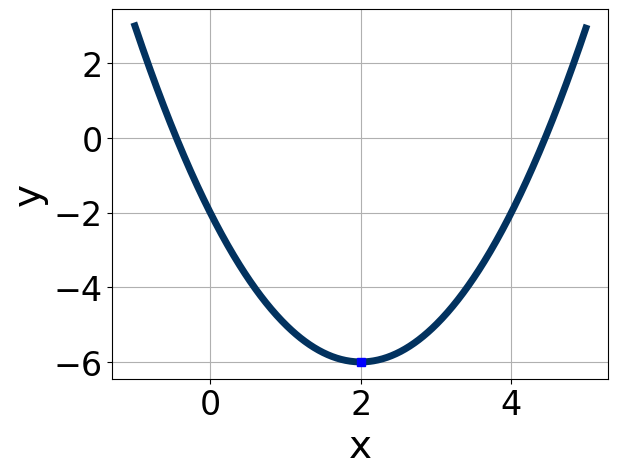
\includegraphics[width=0.5\textwidth]{../Figures/quadraticGraphToEquationB.png}
\end{center}
\begin{enumerate}[label=\Alph*.]
\item \( a \in [-0.1, 2.1], \hspace*{5mm} b \in [-4, 0], \text{ and } \hspace*{5mm} c \in [-4, 1] \)
\item \( a \in [-1.1, -0.9], \hspace*{5mm} b \in [-4, 0], \text{ and } \hspace*{5mm} c \in [-12, -5] \)
\item \( a \in [-1.1, -0.9], \hspace*{5mm} b \in [4, 6], \text{ and } \hspace*{5mm} c \in [-12, -5] \)
\item \( a \in [-0.1, 2.1], \hspace*{5mm} b \in [4, 6], \text{ and } \hspace*{5mm} c \in [-4, 1] \)
\item \( a \in [-0.1, 2.1], \hspace*{5mm} b \in [4, 6], \text{ and } \hspace*{5mm} c \in [7, 14] \)

\end{enumerate} }
\litem{
Graph the equation below.\[ f(x) = (x+3)^2 + 17 \]\begin{enumerate}[label=\Alph*.]
\begin{multicols}{2}\item 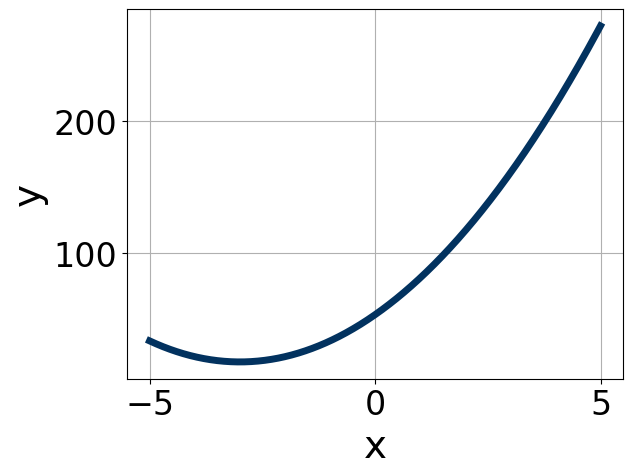
\includegraphics[width = 0.3\textwidth]{../Figures/quadraticEquationToGraphCopyAB.png}\item 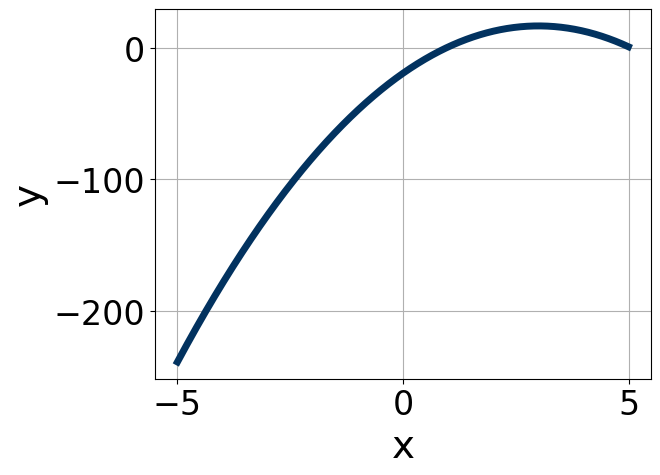
\includegraphics[width = 0.3\textwidth]{../Figures/quadraticEquationToGraphCopyBB.png}\item 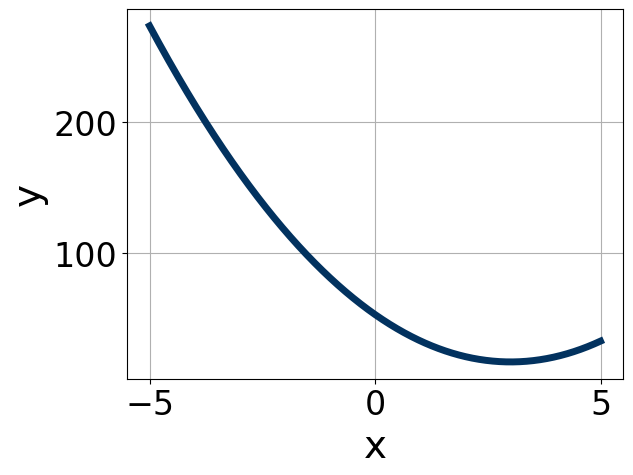
\includegraphics[width = 0.3\textwidth]{../Figures/quadraticEquationToGraphCopyCB.png}\item 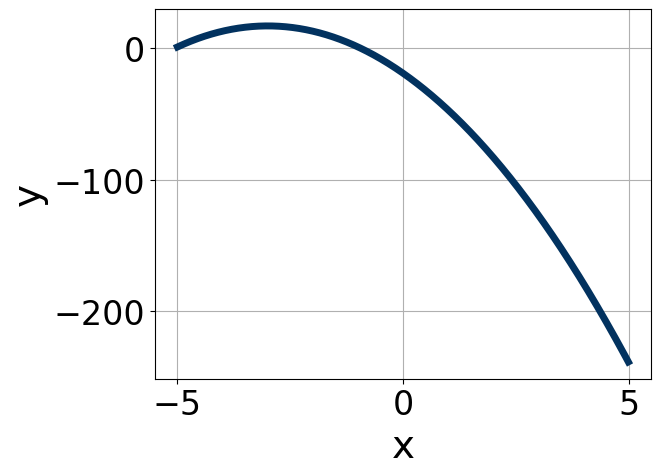
\includegraphics[width = 0.3\textwidth]{../Figures/quadraticEquationToGraphCopyDB.png}\end{multicols}\item None of the above.
\end{enumerate} }
\litem{
Graph the equation below.\[ f(x) = (x-1)^2 + 14 \]\begin{enumerate}[label=\Alph*.]
\begin{multicols}{2}\item 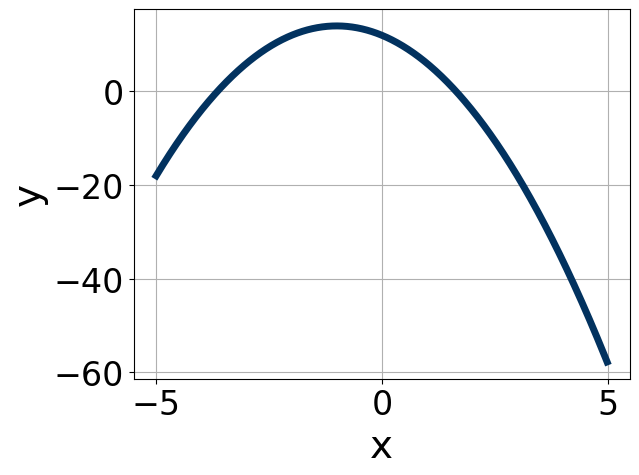
\includegraphics[width = 0.3\textwidth]{../Figures/quadraticEquationToGraphAB.png}\item 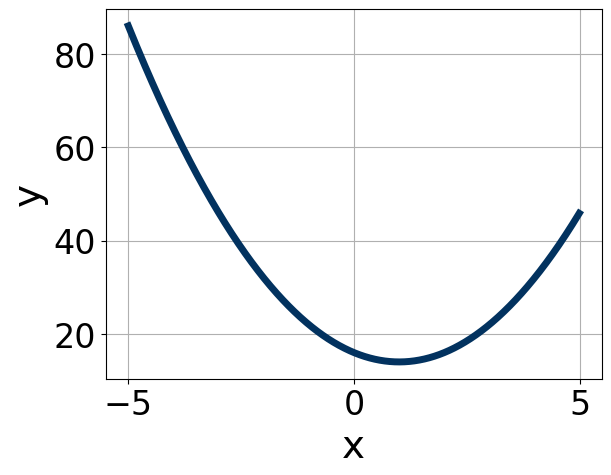
\includegraphics[width = 0.3\textwidth]{../Figures/quadraticEquationToGraphBB.png}\item 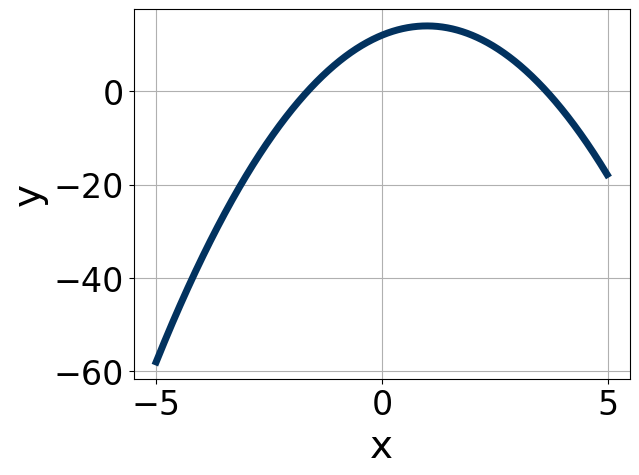
\includegraphics[width = 0.3\textwidth]{../Figures/quadraticEquationToGraphCB.png}\item 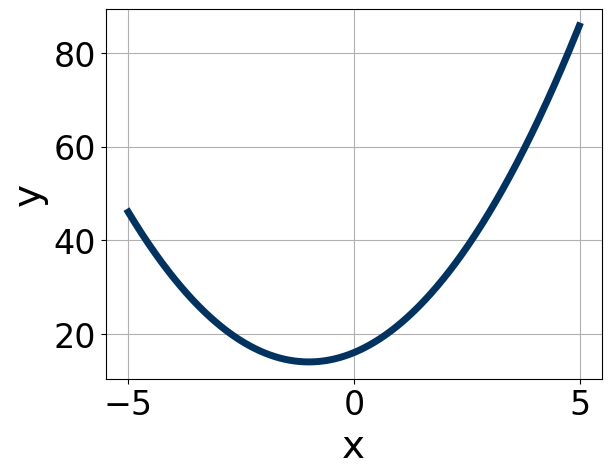
\includegraphics[width = 0.3\textwidth]{../Figures/quadraticEquationToGraphDB.png}\end{multicols}\item None of the above.
\end{enumerate} }
\litem{
Factor the quadratic below. Then, choose the intervals that contain the constants in the form $(ax+b)(cx+d); b \leq d.$\[ 36x^{2} +25 x -25 \]\begin{enumerate}[label=\Alph*.]
\item \( a \in [-1.1, 2.4], \hspace*{5mm} b \in [-21, -15], \hspace*{5mm} c \in [0.67, 1.54], \text{ and } \hspace*{5mm} d \in [39, 49] \)
\item \( a \in [1.4, 4.4], \hspace*{5mm} b \in [-6, -2], \hspace*{5mm} c \in [9.95, 12.66], \text{ and } \hspace*{5mm} d \in [5, 12] \)
\item \( a \in [17.4, 19.4], \hspace*{5mm} b \in [-6, -2], \hspace*{5mm} c \in [1.65, 3.23], \text{ and } \hspace*{5mm} d \in [5, 12] \)
\item \( a \in [7.7, 10.2], \hspace*{5mm} b \in [-6, -2], \hspace*{5mm} c \in [3.99, 4.62], \text{ and } \hspace*{5mm} d \in [5, 12] \)
\item \( \text{None of the above.} \)

\end{enumerate} }
\litem{
Factor the quadratic below. Then, choose the intervals that contain the constants in the form $(ax+b)(cx+d); b \leq d.$\[ 36x^{2} -60 x + 25 \]\begin{enumerate}[label=\Alph*.]
\item \( a \in [2.4, 6.1], \hspace*{5mm} b \in [-6, 0], \hspace*{5mm} c \in [5.7, 7.6], \text{ and } \hspace*{5mm} d \in [-7, -1] \)
\item \( a \in [11.3, 12.4], \hspace*{5mm} b \in [-6, 0], \hspace*{5mm} c \in [1.6, 4.6], \text{ and } \hspace*{5mm} d \in [-7, -1] \)
\item \( a \in [1.3, 2.4], \hspace*{5mm} b \in [-6, 0], \hspace*{5mm} c \in [14.2, 19.6], \text{ and } \hspace*{5mm} d \in [-7, -1] \)
\item \( a \in [-1, 1.3], \hspace*{5mm} b \in [-39, -26], \hspace*{5mm} c \in [0.4, 2.2], \text{ and } \hspace*{5mm} d \in [-31, -29] \)
\item \( \text{None of the above.} \)

\end{enumerate} }
\litem{
Write the equation of the graph presented below in the form $f(x)=ax^2+bx+c$, assuming  $a=1$ or $a=-1$. Then, choose the intervals that $a, b,$ and $c$ belong to.
\begin{center}
    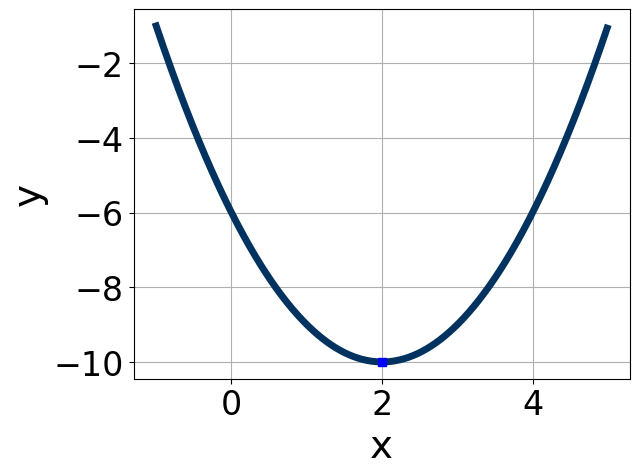
\includegraphics[width=0.5\textwidth]{../Figures/quadraticGraphToEquationCopyB.png}
\end{center}
\begin{enumerate}[label=\Alph*.]
\item \( a \in [0, 2.1], \hspace*{5mm} b \in [4, 5], \text{ and } \hspace*{5mm} c \in [12, 16] \)
\item \( a \in [0, 2.1], \hspace*{5mm} b \in [-5, -3], \text{ and } \hspace*{5mm} c \in [-10, -5] \)
\item \( a \in [-2.4, -0.4], \hspace*{5mm} b \in [4, 5], \text{ and } \hspace*{5mm} c \in [-18, -12] \)
\item \( a \in [0, 2.1], \hspace*{5mm} b \in [4, 5], \text{ and } \hspace*{5mm} c \in [-10, -5] \)
\item \( a \in [-2.4, -0.4], \hspace*{5mm} b \in [-5, -3], \text{ and } \hspace*{5mm} c \in [-18, -12] \)

\end{enumerate} }
\litem{
Solve the quadratic equation below. Then, choose the intervals that the solutions belong to, with $x_1 \leq x_2$ (if they exist).\[ -20x^{2} -12 x + 7 = 0 \]\begin{enumerate}[label=\Alph*.]
\item \( x_1 \in [-28.21, -26.58] \text{ and } x_2 \in [25.01, 26.46] \)
\item \( x_1 \in [-2.16, -0.63] \text{ and } x_2 \in [-0.8, 0.6] \)
\item \( x_1 \in [-7.95, -7.16] \text{ and } x_2 \in [18.61, 19.61] \)
\item \( x_1 \in [-0.83, -0.32] \text{ and } x_2 \in [0.83, 1.8] \)
\item \( \text{There are no Real solutions.} \)

\end{enumerate} }
\litem{
Solve the quadratic equation below. Then, choose the intervals that the solutions $x_1$ and $x_2$ belong to, with $x_1 \leq x_2$.\[ 20x^{2} -69 x + 54 = 0 \]\begin{enumerate}[label=\Alph*.]
\item \( x_1 \in [1.18, 1.23] \text{ and } x_2 \in [1.78, 2.38] \)
\item \( x_1 \in [0.72, 0.8] \text{ and } x_2 \in [2.26, 4.68] \)
\item \( x_1 \in [0.43, 0.57] \text{ and } x_2 \in [5.49, 6.16] \)
\item \( x_1 \in [0.34, 0.43] \text{ and } x_2 \in [6.06, 8.15] \)
\item \( x_1 \in [23.98, 24.13] \text{ and } x_2 \in [44.97, 46.05] \)

\end{enumerate} }
\litem{
Solve the quadratic equation below. Then, choose the intervals that the solutions $x_1$ and $x_2$ belong to, with $x_1 \leq x_2$.\[ 15x^{2} +47 x + 36 = 0 \]\begin{enumerate}[label=\Alph*.]
\item \( x_1 \in [-10.8, -6.8] \text{ and } x_2 \in [-0.33, 0.07] \)
\item \( x_1 \in [-29.4, -24.2] \text{ and } x_2 \in [-20.1, -19.75] \)
\item \( x_1 \in [-6.4, -4.8] \text{ and } x_2 \in [-0.71, -0.42] \)
\item \( x_1 \in [-3.7, -1.9] \text{ and } x_2 \in [-0.92, -0.68] \)
\item \( x_1 \in [-1.9, 0.5] \text{ and } x_2 \in [-1.41, -1.1] \)

\end{enumerate} }
\litem{
Solve the quadratic equation below. Then, choose the intervals that the solutions belong to, with $x_1 \leq x_2$ (if they exist).\[ -16x^{2} -9 x + 3 = 0 \]\begin{enumerate}[label=\Alph*.]
\item \( x_1 \in [-0.6, 0.5] \text{ and } x_2 \in [0.3, 3.9] \)
\item \( x_1 \in [-17.6, -16.6] \text{ and } x_2 \in [14.4, 17.6] \)
\item \( x_1 \in [-5.8, -1.5] \text{ and } x_2 \in [11.3, 14.1] \)
\item \( x_1 \in [-2.1, -0.5] \text{ and } x_2 \in [-0.9, 0.3] \)
\item \( \text{There are no Real solutions.} \)

\end{enumerate} }
\end{enumerate}

\end{document}